\documentclass{beamer}
\usepackage{comment}
\usepackage{tikz}

\title{Tallahassee Crime Map}
\author{Munawar Ali, Çağatay Ayhan, Ece Karaçam, Abdullah Malik, and Mao Nishino}

\date{\today}

\begin{document}

\begin{frame}
    \titlepage
\end{frame}

\begin{frame}
    \frametitle{Outline}
    \tableofcontents
\end{frame}

%%% Keep the hourly bar-chart
%% add the location bar-chart

\section{Introduction}
\begin{frame}{Project At A Glance}

    % Use columns to separate the text from the images
    \begin{columns}[T] % The [T] alignment option aligns the columns content at the top

        \begin{column}{.5\textwidth}
            \textbf{Goal:} Develop a generative AI that outputs a crime distribution given a geographical map.\\
            \quad \\
            \textbf{Why:} To provide a tool for city planners to see potential crime risks with their plans.\\
            \quad \\
            \textbf{Technology:} Generative Adversarial Network (pix2pix)
        \end{column}

        \begin{column}{.5\textwidth}
            \begin{figure}
                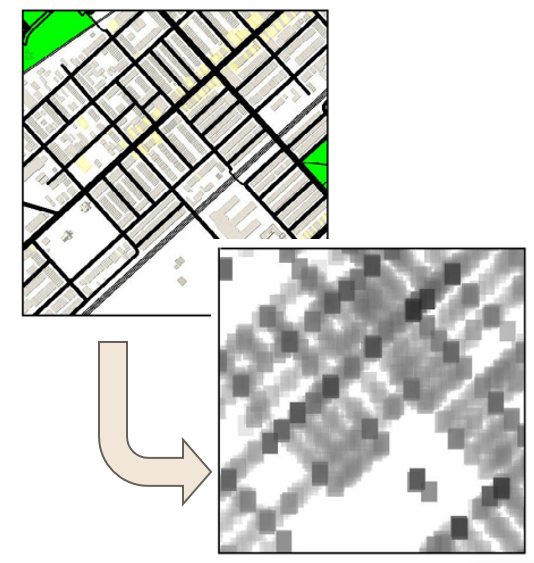
\includegraphics[width=\textwidth]{Figures/Intro Figure.png} % Replace with the path to your map image
                \caption{Geographical Map to Crime Map(Adapted from He, Zheng 2021)}
            \end{figure}
        \end{column}

    \end{columns}

\end{frame}

\section{Data Collection and Processing}
\begin{frame}
    \frametitle{TOPS Data Collection}
    \begin{columns}[T] % align columns
        \begin{column}{.48\textwidth}
            % Image block
            \begin{figure}
                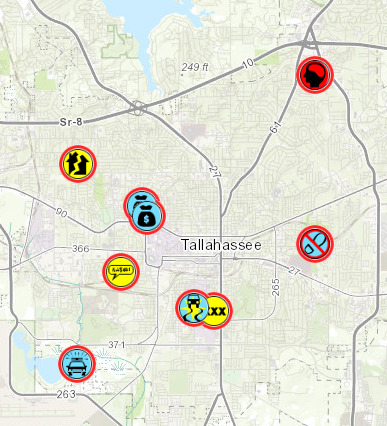
\includegraphics[width=\linewidth]{Figures/TOPS.png} % replace with your image path
                % Set a label for the image to refer to it later
                \label{fig:tops}
                \caption{Tallahasse Police Statistics Homepage}
            \end{figure}
        \end{column}%

        \begin{column}{.48\textwidth}
            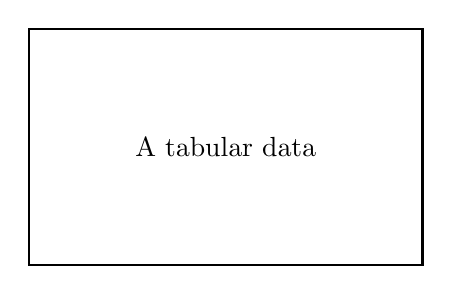
\begin{tikzpicture}
                \node[rectangle, draw=black, thick, minimum width=5cm, minimum height=3cm, text centered] (table) {A tabular data};
            \end{tikzpicture}
            The table contains the following columns:
            \begin{itemize}
                \item Time of the crime report
                \item Crime type
                \item Location
                \item Geographical coordinates
            \end{itemize}
        \end{column}%
    \end{columns}

    % Draw an arrow from the image to the table using TikZ
    \begin{tikzpicture}[overlay, remember picture]
        % Define the starting point of the arrow at the bottom of the image
        \coordinate (image) at ([xshift=3cm]current page.west);
        % Define the ending point of the arrow at the top of the table
        \coordinate (table) at ([xshift=-5cm, yshift=2cm]current page.east);

        % Draw the arrow
        \draw[->, draw=blue, line width=0.5cm, in=180] (image) to (table);
    \end{tikzpicture}
\end{frame}

\begin{frame}
    \frametitle{Data Processing}
    Write a short description about how we create our map dataset
\end{frame}

%%%%%%%%%%%%%%%%%%%%%%%%%%% SPATIAL ANALYSIS BEGIN %%%%%%%%%%%%%%%%%%%%%

\begin{frame}
    \frametitle{Categorical Analysis}
    \begin{minipage}[c]{0.65\textwidth}
        \begin{figure}
            \centering
            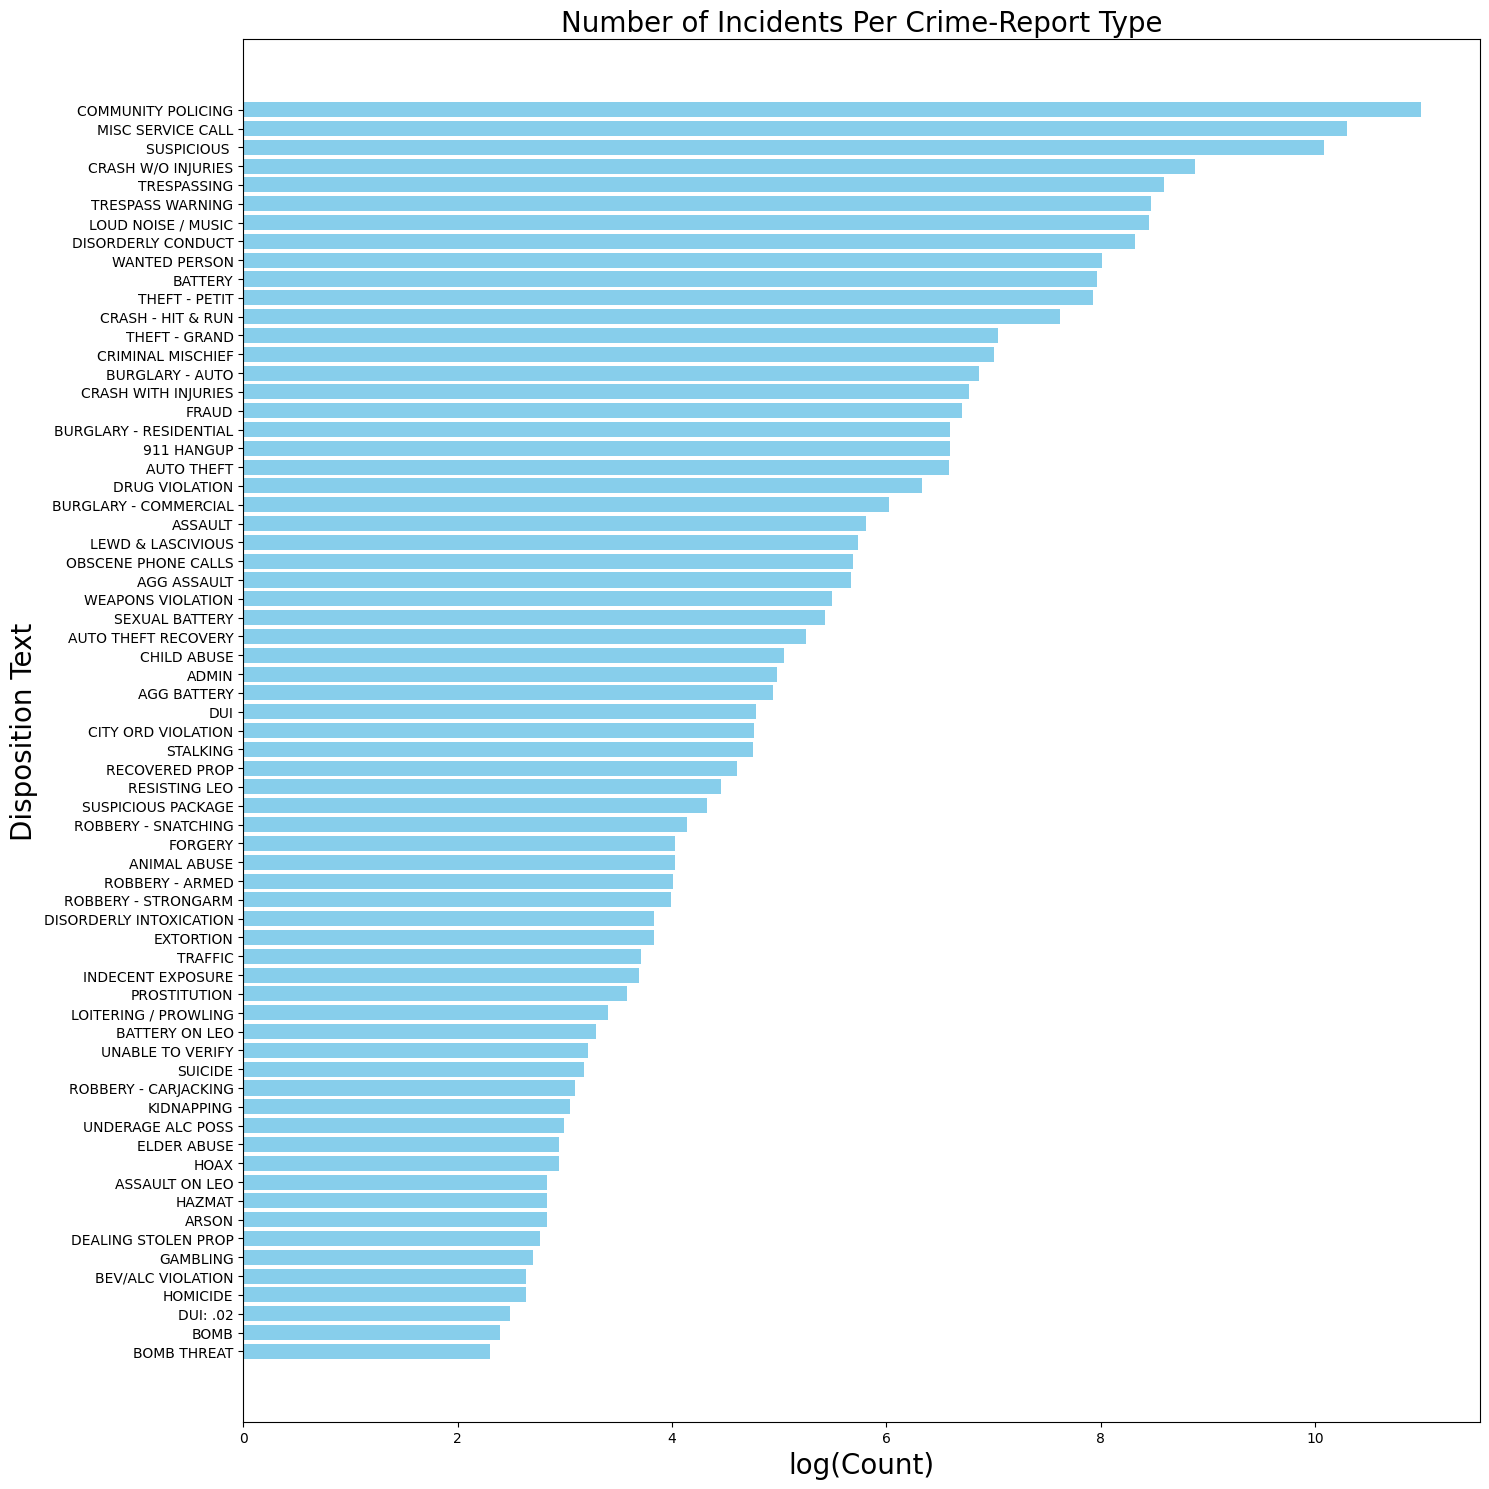
\includegraphics[width=\linewidth]{Figures/Number of Incidents Per Crime-Report Type.png}
            \caption{A bar chart for each type of crime report.}
        \end{figure}
    \end{minipage}\hfill
    \begin{minipage}[c]{0.3\textwidth}
        {\scriptsize % Smaller text to fit more content
            \begin{itemize}
                \item The values on the $x$-axis correspond to the log of the actual count for visual purposes.
                \item On the $y$-axis all different types of crime reports are listed.
                \item There are 67 types of reports.
                \item We will filter out some from our analysis. For example, community policing occurs most often and it is not of interest for our purposes.
            \end{itemize}
        }
    \end{minipage}
\end{frame}








%%%%%%%%%%%%%%%%%%%%%%%%%%% SPATIAL ANALYSIS END %%%%%%%%%%%%%%%%%%%%%%%


%%%%%%%%%%%%%%%%%%%%%%%%%%% TEMPORAL ANALYSIS BEGIN%%%%%%%%%%%%%%%%%
\section{Experimental Data Analysis}


\begin{comment}
\begin{frame}
    \frametitle{Temporal Analysis}
    % Put figures about temporal trends in crime data (per semester, per month, per day, per hour, etc.)
    \begin{minipage}[c]{0.7\textwidth}
        \begin{figure}
            \centering
            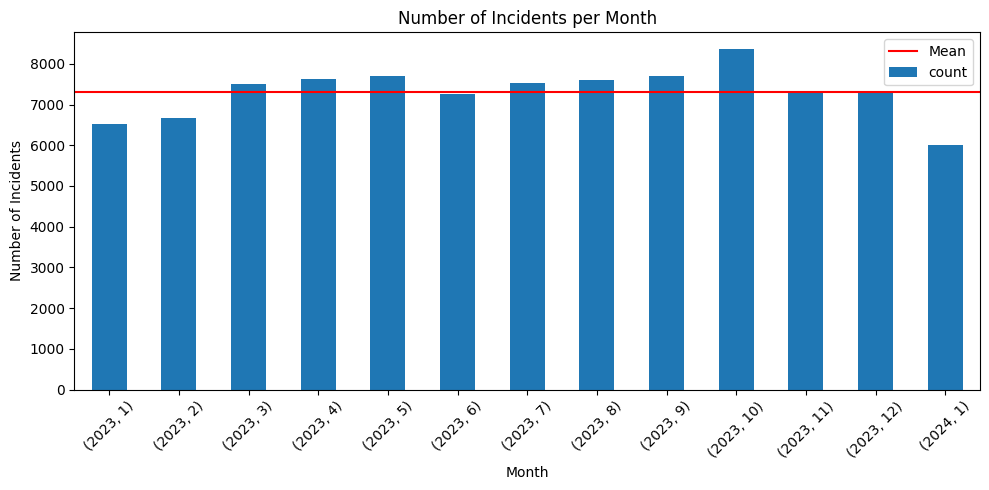
\includegraphics[width=\linewidth]{Figures/Number of Incidents Per Month.png}
            \caption{Crime Distribution Per Month}
        \end{figure}
    \end{minipage}\hfill
    \begin{minipage}[c]{0.3\textwidth}
        {\scriptsize % Smaller text to fit more content
            \begin{itemize}
                \item Average \# of reported crimes per month is $7311$.
                \item Data includes all of 2023 and the first month of 2024.
            \end{itemize}
        }
    \end{minipage}

\end{frame}
\end{comment}

%%%%%%%%%%%%%%%%%%%%%%%%%%% Temporal Analysis Page 2 %%%%%%
\begin{frame}
    \frametitle{Temporal Analysis}
    % Put figures about temporal trends in crime data (per semester, per month, per day, per hour, etc.)
    \begin{minipage}[c]{0.7\textwidth}
        \begin{figure}
            \centering
            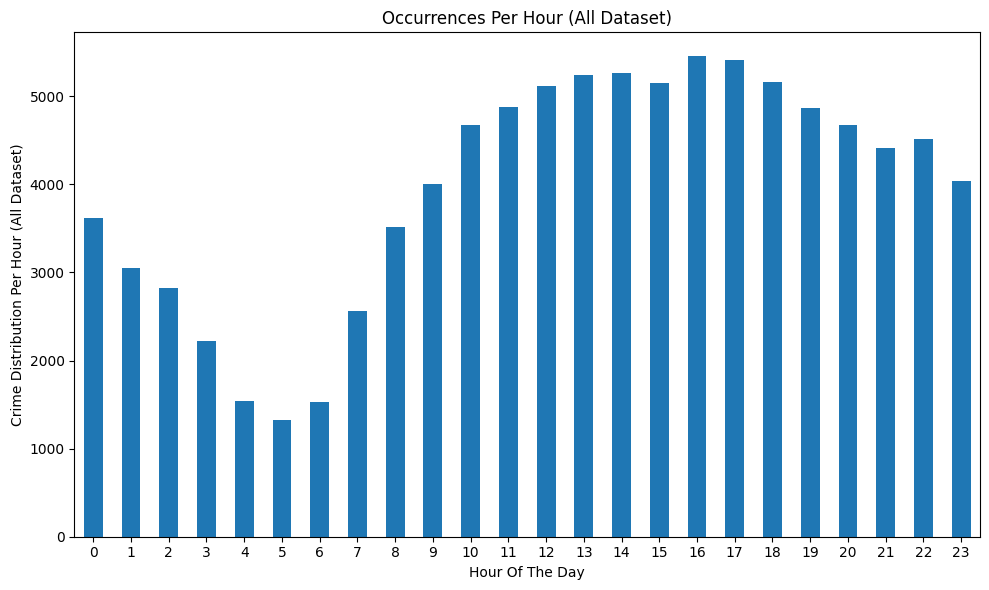
\includegraphics[width=\linewidth]{Figures/Crime Distribution Per Hour (All Dataset).png}
            \caption{Crime Distribution Per Hour -- All 2023}
        \end{figure}
    \end{minipage}\hfill
    \begin{minipage}[c]{0.3\textwidth}
        {\scriptsize % Smaller text to fit more content
            \begin{itemize}
                \item Hourly analysis of the data reveals a fluctuating trend with peak hours.
                \item Data includes all of 2023.
            \end{itemize}
        }
    \end{minipage}

\end{frame}

%%%%%%%%%%%%%%%%%%%%%%%%%%% Temporal Analysis Page 3 %%%%%%

\begin{comment}

\begin{frame}
    \frametitle{Temporal Analysis}
    % Put figures about temporal trends in crime data (per semester, per month, per day, per hour, etc.)
    \begin{figure}
        \flushleft
        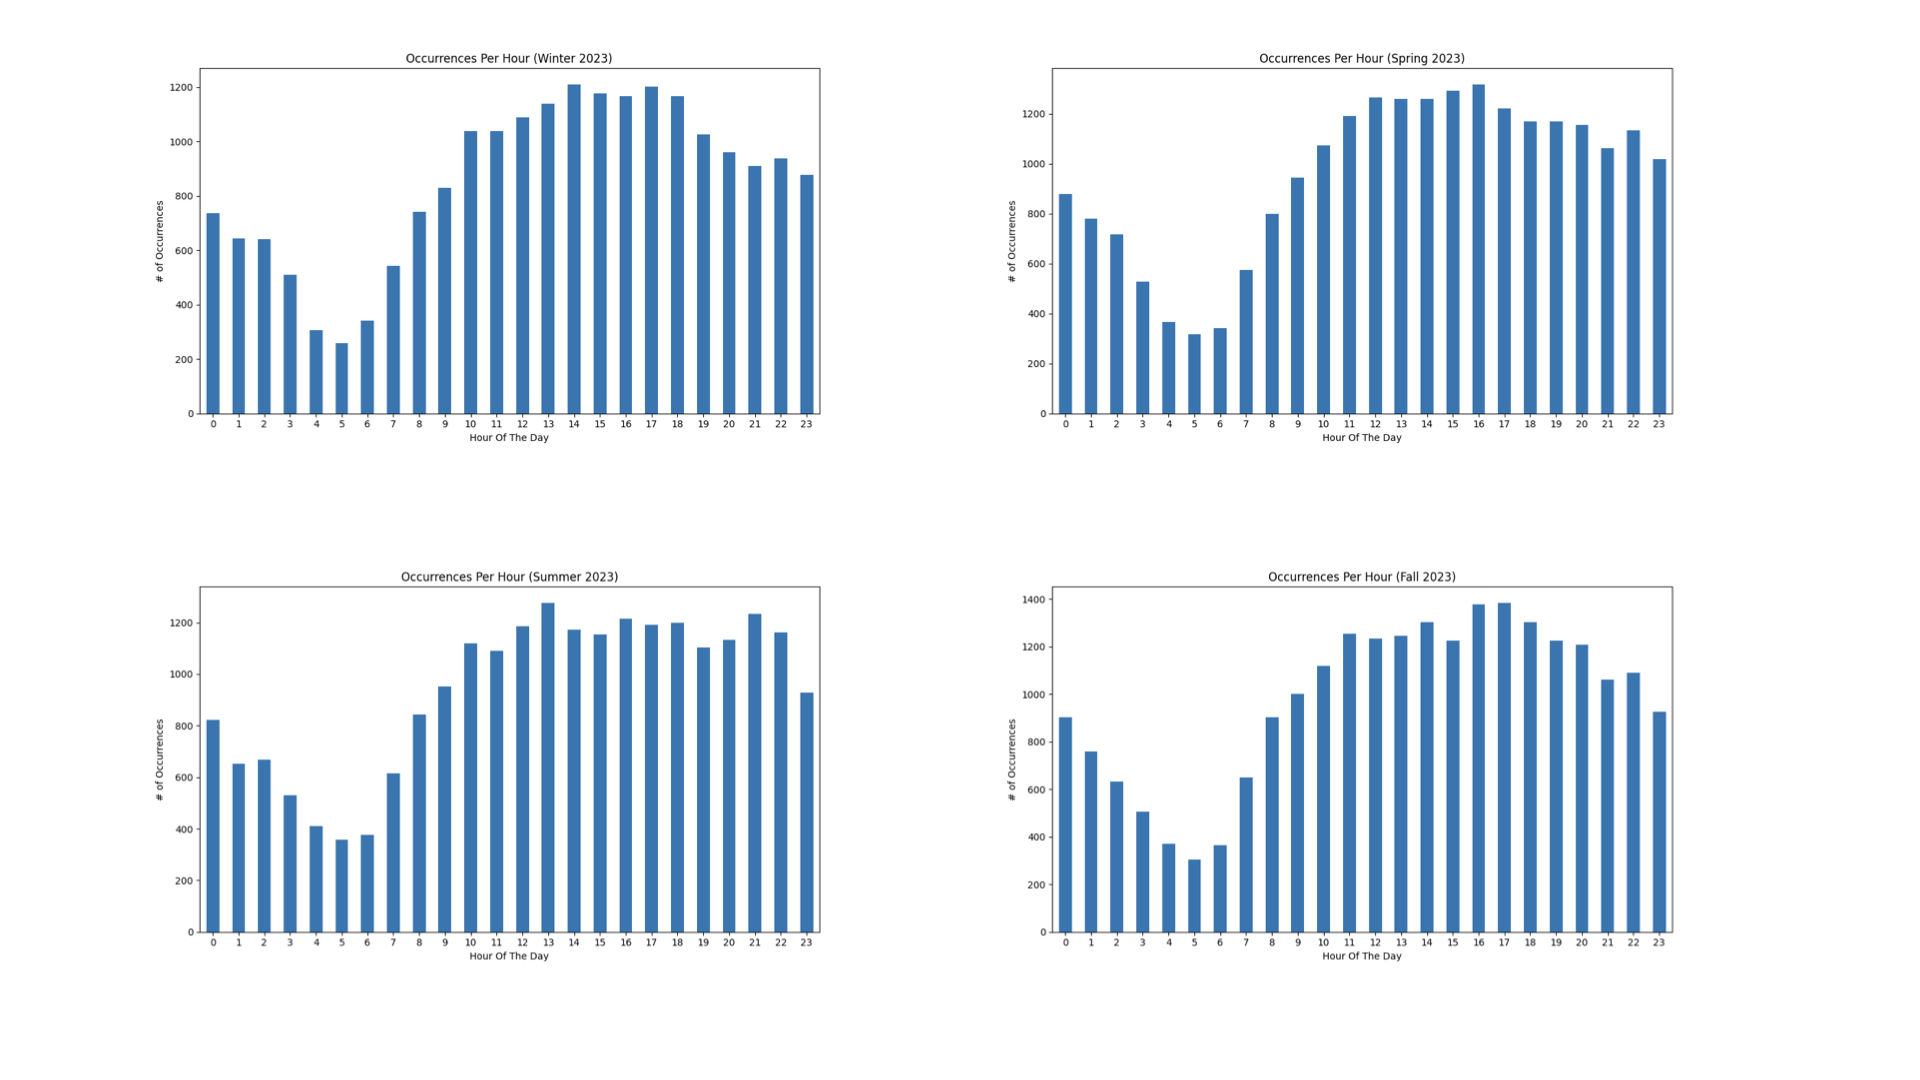
\includegraphics[width=1\linewidth]{Figures/OccurencesPerSeason.001.jpeg}
    \end{figure}
    {\scriptsize % Smaller text to fit more content
    \begin{itemize}
        \item  Hourly crime distribution using portions of the data.
        \item  Same trend across different seasons of the year 2023.
    \end{itemize}
    }


\end{frame}
\end{comment}

%%%%%%%%%%%%%%%%%%%%%%%%%%% Temporal Analysis Page 4 %%%%%%

\begin{frame}
    \frametitle{Temporal Analysis}
    % Put figures about temporal trends in crime data (per semester, per month, per day, per hour, etc.)
    \begin{figure}
        \flushleft
        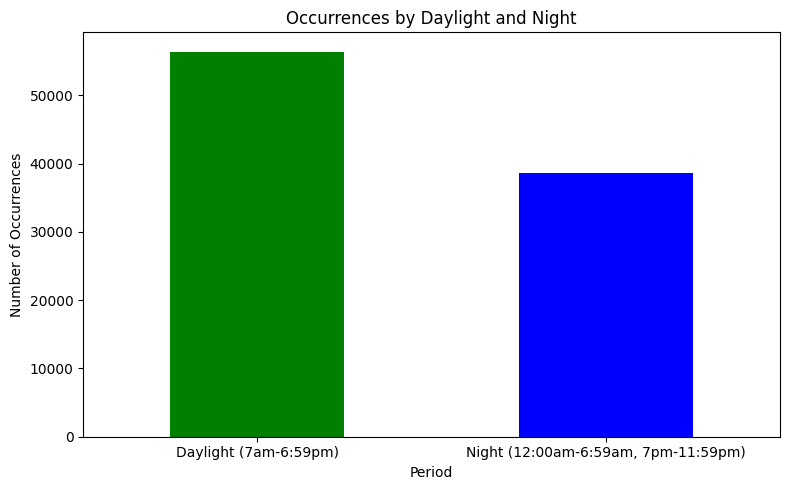
\includegraphics[width=1\linewidth]{Figures/Daylight_and_Night.png}
    \end{figure}
    {\scriptsize % Smaller text to fit more content
    \begin{itemize}
        \item  Daylight vs no daylight. When is an incident more likely to occur?
    \end{itemize}
    }
\end{frame}




%%%%%%%%%%%%%%%%%%%%%%%%%%% Temporal Analysis Page 5 %%%%%%

\begin{comment}
\begin{frame}
    \frametitle{Temporal Analysis}
    % Put figures about temporal trends in crime data (per semester, per month, per day, per hour, etc.)
    \begin{figure}
        \flushleft
        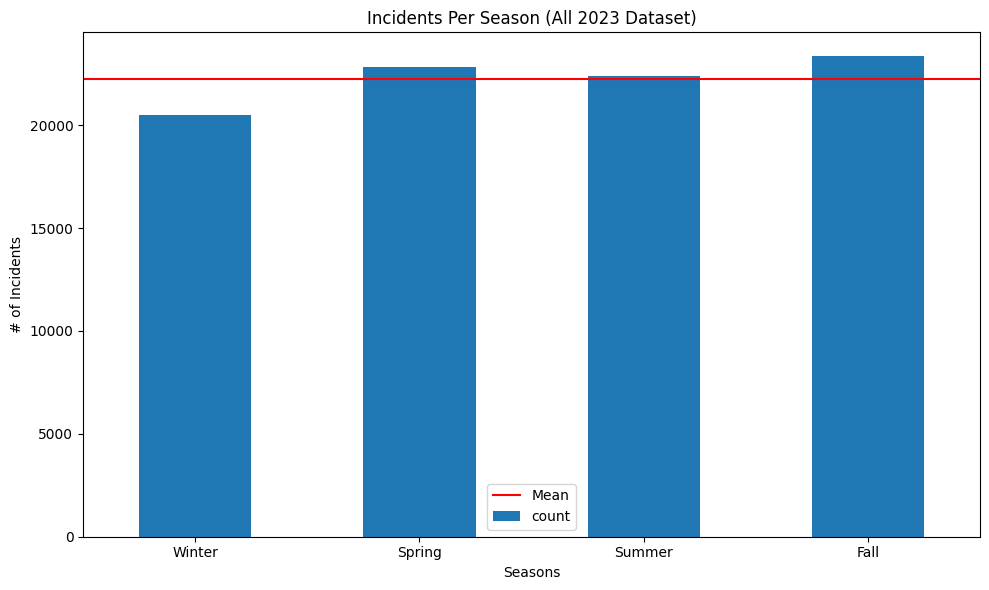
\includegraphics[width=1\linewidth]{Figures/Incidents Per Season (All 2023 Dataset).png}
    \end{figure}
    {\scriptsize % Smaller text to fit more content
    \begin{itemize}
        \item  Crime-report distribution based on seasons.
    \end{itemize}
    }
\end{frame}
\end{comment}

%%%%%%%%%%%%%%%%%%%%%%%%%%% Temporal Analysis Page 6 %%%%%%

\begin{frame}
    \frametitle{Temporal Analysis}
    % Put figures about temporal trends in crime data (per semester, per month, per day, per hour, etc.)
    \begin{figure}
        \flushleft
        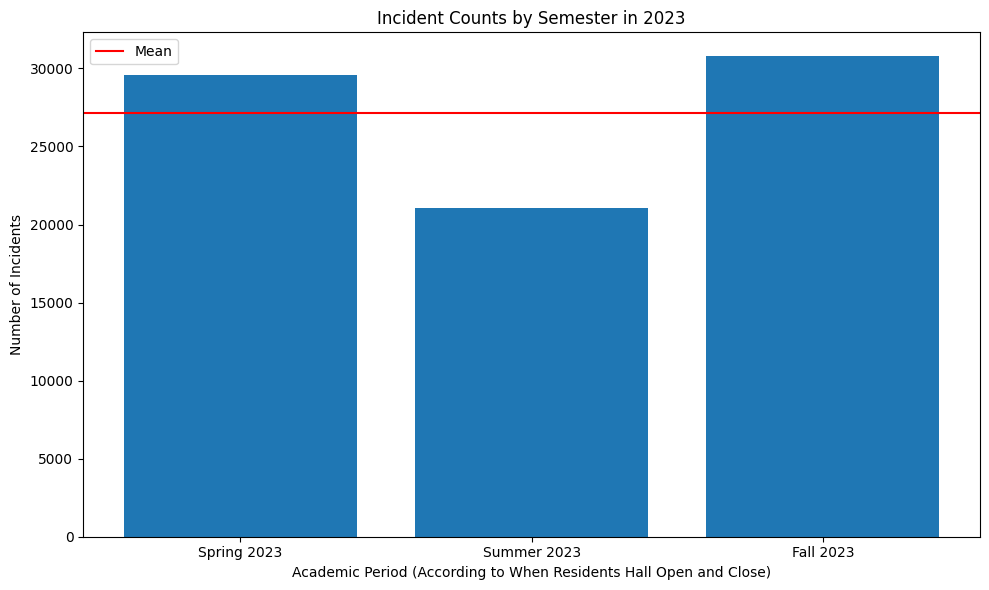
\includegraphics[width=1\linewidth]{Figures/Incident Counts by Semester in 2023.png}
    \end{figure}
    {\scriptsize % Smaller text to fit more content
    \begin{itemize}
        \item Tallahassee is a college town. (FSU \& FAMU \& TCC)
        \item Do students affect the number of crime reports?
    \end{itemize}
    }
\end{frame}


%%%%%%%%%%%%%%%%%%%%%%%%%%% TEMPORAL ANALYSIS END%%%%%%%%%%%%%%%%%%



\section{Crime Heatmap Generation}

\begin{frame}
    \frametitle{What is Generative Adversarial Network-GAN?}
    \begin{figure}
        \centering
        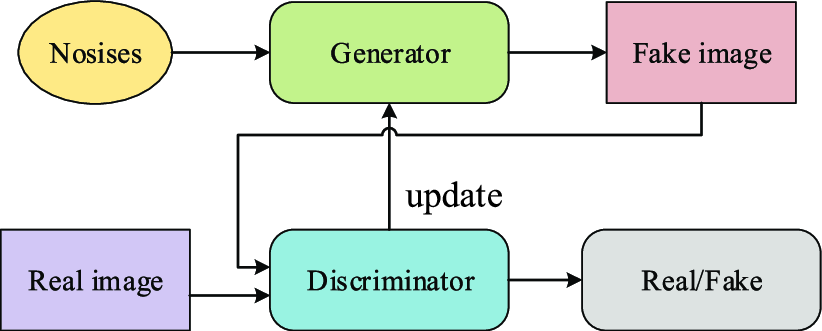
\includegraphics[width=10cm]{Figures/GAN.png}
        \caption{GAN}
        \label{gan}
    \end{figure}
    In the training, $G$ and $D$ try to beat each other (hence the word “adversarial”).\\
    The training stops when $D$ can no longer discriminate fake samples.

\end{frame}


\begin{frame}
    \frametitle{Conditional GAN (Pix2pix)}
    What do we do if we want a G network that takes a geographical map and outputs a crime map?
    \begin{figure}
        \centering
        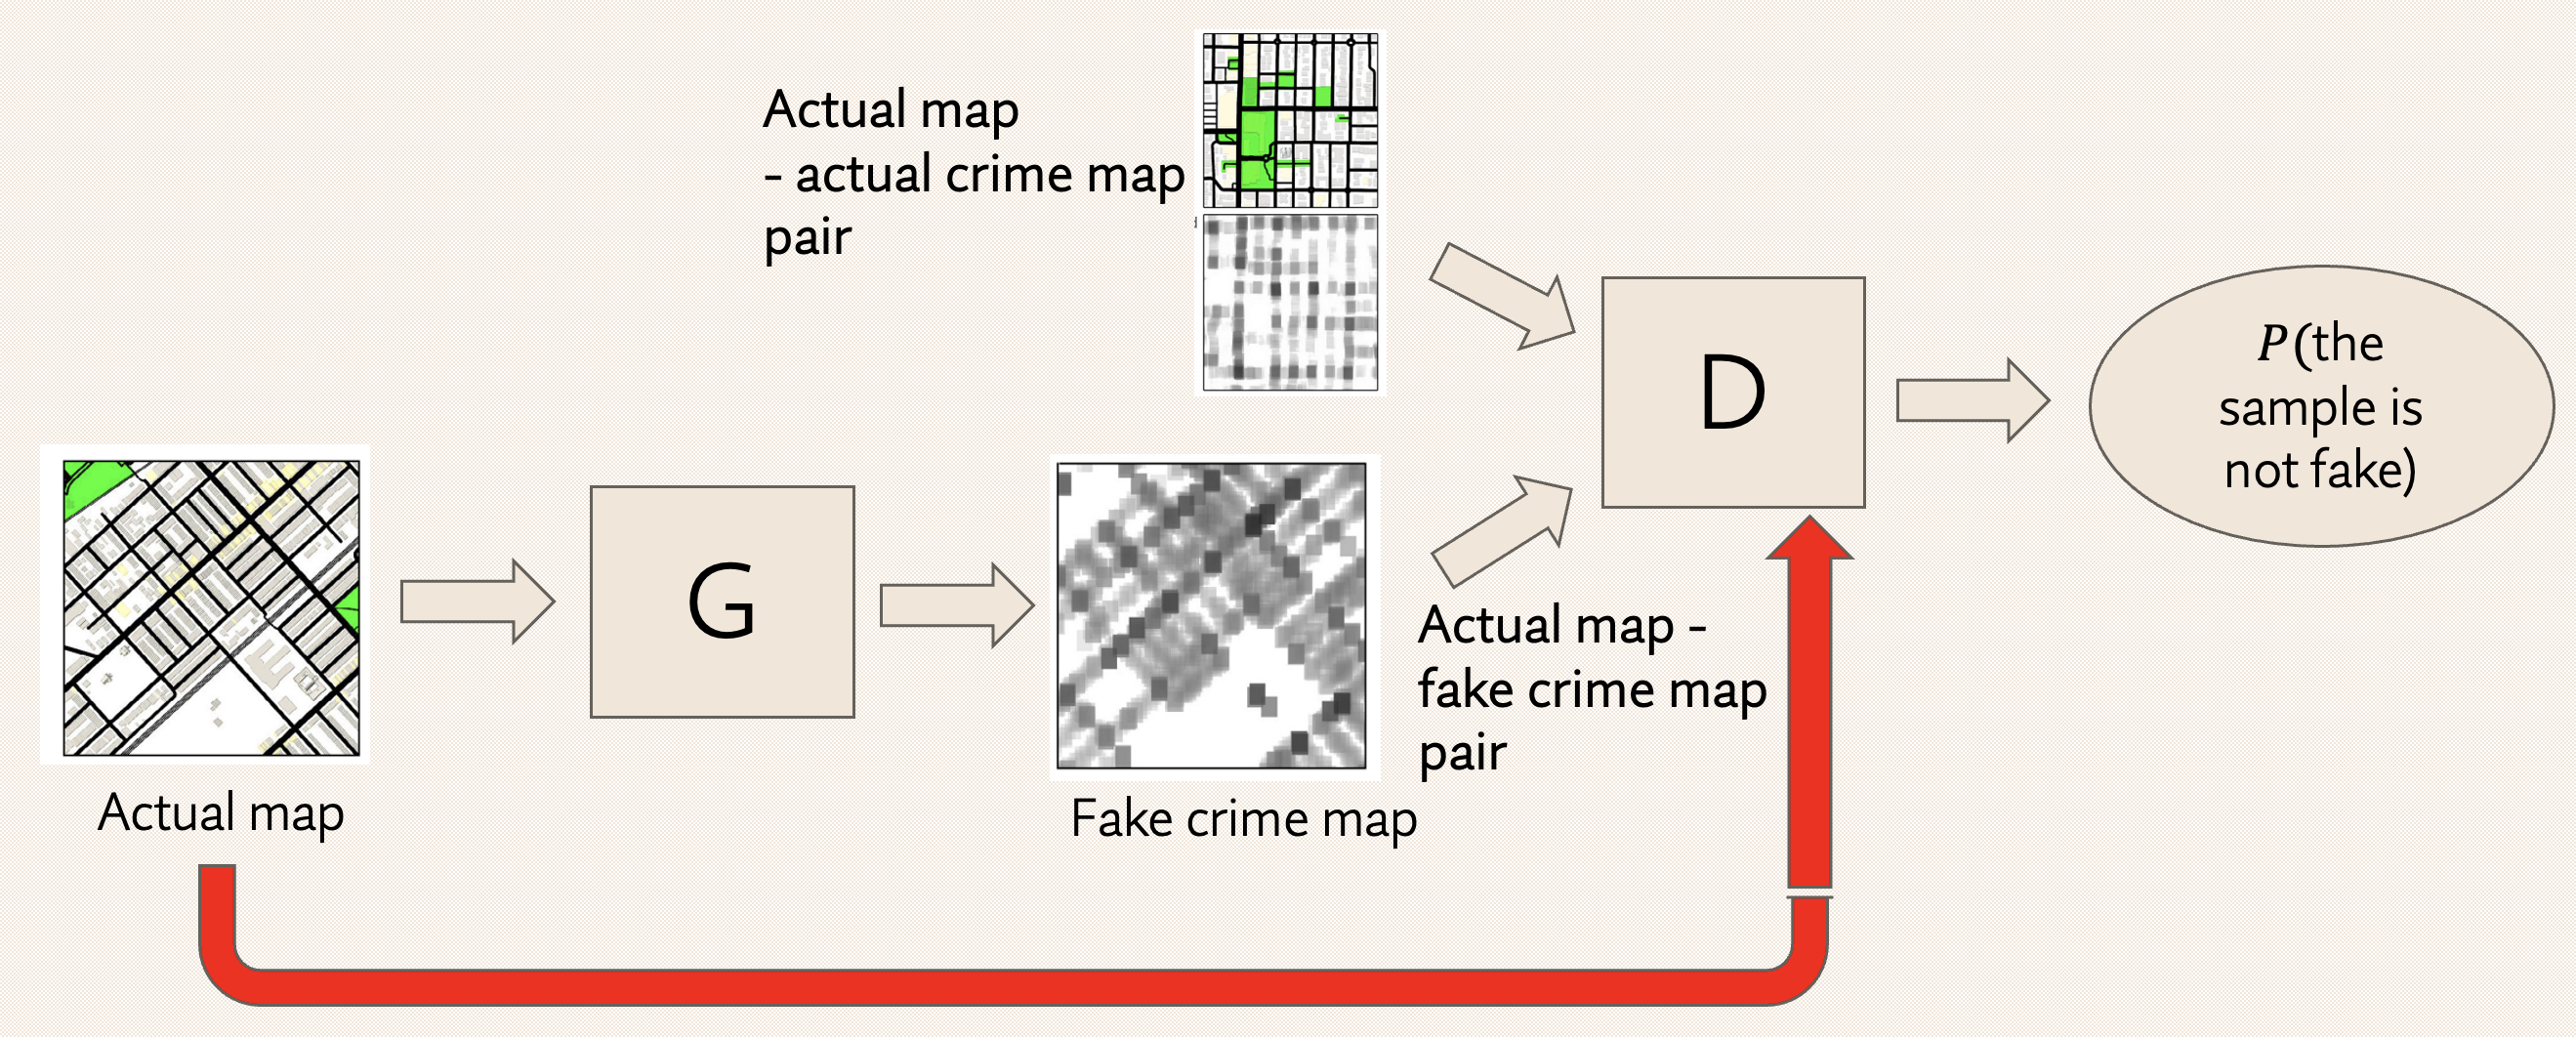
\includegraphics[width=11cm]{Figures/conditionalgan.png}
        \caption{pix2pix}
        \label{pix2pix}
    \end{figure}

    After training, a crime map generator is born.
\end{frame}

\begin{frame}{Results} % Add your frame title here

    % Wide block at the top
    \begin{figure}
        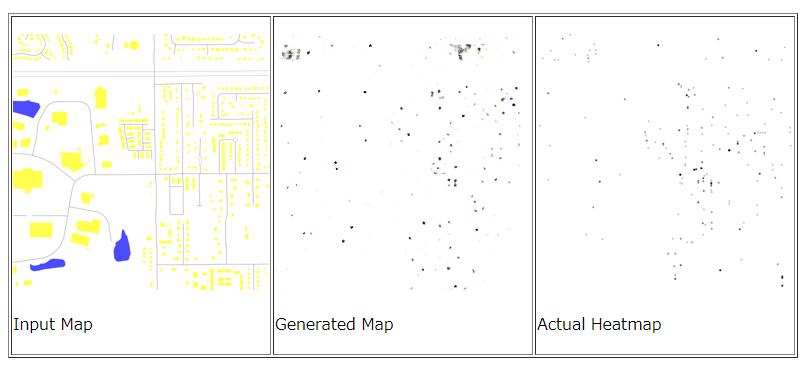
\includegraphics[width=0.8\linewidth]{Figures/Generated heats.png} % Replace with the path to your image
        \caption{Generated heatmaps. We observe that the spatial pattern is somewhat similar to the real data.}
    \end{figure}

    \begin{table}[]
        \begin{tabular}{|l|l|l|}
            \hline
                        & Baseline (Random Points) & pix2pix            \\ \hline
            Average MSE & 3.9543179869651794       & 0.9491354823112488 \\ \hline
        \end{tabular}
    \end{table}
\end{frame}

\section{Conclusion}
\begin{frame}
    \frametitle{Conclusion}
    \begin{itemize}
        \item The data shows interesting trends in both spatial and temporal dimensions.
        \item In particular, the absense of students during the summer months is reflected in the crime reports.
        \item Using pix2pix, we were able to generate heatmaps that resemble the real data.
        \item In future, we can do:
        \item \quad Better training of the model
        \item \quad Implement a user-friendly editor for georaphical maps for hypothetical maps
        \item \quad Implement a web-app for the tool
    \end{itemize}
\end{frame}

\begin{frame}
    \frametitle{Thank You}
    \centering
    \Huge Thank You!
\end{frame}

\end{document}